\documentclass[a4paper,10pt]{article}

\usepackage{amsmath}%
\usepackage{amsfonts}%
\usepackage{amssymb}%
\usepackage{graphicx}
\usepackage{subfigure}
\usepackage{algorithmic}
\usepackage{listings}
%\usepackage{hyperref}
 
%opening
\title{Gabor-Boosting Face Recognition}
\author{Mian Zhou and Hong Wei\\
\small School of System Engineering\\[-0.8ex]
\small University of Reading\\
\small Reading RG6 6AY\\
\small United Kingdom\\
\small \texttt{m.zhou, h.wei@reading.ac.uk}
% \and
% Hong Wei\\
% \small School of System Engineering\\[-0.8ex]
% \small University of Reading, Reading RG6 6AY, United Kingdom\\
% \small \texttt{h.wei@reading.ac.uk}
}



\begin{document}

\maketitle

% \par
% {\textbf{Corresponding Author}\\
% Mian Zhou\\
% \small School of System Engineering\\[-0.8ex]
% \small University of Reading, Reading RG6 6AY, United Kingdom\\
% \small Telephone: +44 (0) 118 378 8608, Fax: +44 (0) 118 975 1822\\
% \small \texttt{m.zhou@reading.ac.uk}
% }

\begin{abstract}
In this paper, we present an accurate appearance-based face recognition algorithm with Gabor wavelet transform for feature extraction, AdaBoosting algorithm for feature selection, and Support Vector Machine (SVM) for classification. Within the AdaBoost algorithm, we design a novel weak learner - Potsu which is the only weak learner fulfilling the requirement of AdaBoost. In classification, we found that ensemble classifier made from AdaBoost may prone to overfitting, and the effects can be reduce by SVM.\\

\textbf{Keywords:} Face Recognition, Gabor Wavelets, AdaBoost, SVM
\end{abstract}


%\newpage
%\tableofcontents
\section{Introduction}
\label{intro}
In recent years, biometrics has been used to identify individuals using traits based on retina, iris, fingerprints, or face. Personal identification based on face images is of particular interest as they are non invasive and rely lessly on the cooperation of the individual. 

Depending on the application context, face recognition is divided into two scenarios: face verification and face identification. In face verification, an individual who desires to be recognised claims an identity, usually through a personal identification number, an user name, or a smart card, so that face verification is to answer question - ``Does the face belong to the specified person?''. In face identification, the system is to establish an individual's identity without the subject to claim an identity, so that face identification is to answer question - ``Whose face is this?''.

The face recognition system presented in this paper is based on individual subject in a way of face verification. Face verification in this paper is to verify a claimed identity by face image of the individual, and a classifier labels the image as two classes, i.e. client or impostor \cite{zhou2006icpr}. A client is the given individual with claimed identity. Impostors are all other persons except the client. In this way, the face verification can be defined as client-based. By specifying a certain person, all face images belonging to the person are recognised as the client, others are recognised as impostors. In terms of machine learning, the client is considered as positive examples, and impostors are considered as negative examples. For such a two-class classification , techniques developed for object detection and face detection \cite{Viola2001,Viola2004} can be used.

The face recognition process consists of three phases: feature extraction, feature selection and classification. Feature extraction is to construct a high dimensional feature space from the image space. Feature selection reduces the dimensionality of the feature space, and spans a low dimensional subspace. Classification verifies a new face image as a client or an impostor. In this paper, we present a new face recognition algorithm called Gabor-Boosting, which is motivated by Boosting face detection \cite{Viola2001} and Gabor wavelet representation. Gabor wavelet transform is used to extract Gabor wavelet features from face images. Due to very large number of features available, AdaBoost is used to select small group of features representing individual face. Finally, the verification is conducted by Support Vector Machine (SVM) classifiers with selected features. To evaluate the performance of Gabor-Boosting algorithm, the \mbox{XM2VTS} face database is used.

The paper is organised as follows: \mbox{Section} \ref{feature_extraction} describes the Gabor wavelet feature extraction; \mbox{Section} \ref{feature_selection} presents the feature selection algorithm, in which a novel weak learner - Potsu is proposed; two types of classification are explored in \mbox{Section} \ref{classification}, i.e. ensemble and SVM classification. It has shown that SVM is appropriate for classification in Gabor-Boosting; and finally \mbox{Section} \ref{conclusion} gives the conclusion.


\section{Gabor Wavelet Feature Extraction}
\label{feature_extraction}
This section discusses the Gabor wavelets and how face images are represented by Gabor wavelet features. Firstly, the background of Gabor wavelets is given. Secondly, the Gabor wavelet and its parameters are defined. Thirdly, Gabor wavelet transform is illustrated and the representatives of face images - Gabor wavelet features are presented.

\subsection{Background of Gabor Wavelet}
Gabor wavelets exhibit desirable characteristics of spatial locality and orientation selectivity. Their kernels are similar to the two-dimensional (2-D) receptive field profiles of the mammalian cortical simple cells \cite{Hubel1978}. Gabor wavelets capture the local structure corresponding to spatial frequency\footnote{In somewhere, spatial frequency is referred as scale.}, spatial localisation, and orientation selectivity. As a result, Gabor wavelet representation of face images is robust to variations due to illumination and facial expression changes \cite{Olshausen1996,Rao1995,Schiele2000}. 

Two-dimensional Gabor wavelets are first introduced into biometric research by Daugman \cite{Daugman1993} for human iris recognition. Lades et al \cite{Lades1993} apply Gabor wavelets in face recognition using the Dynamic Link Architecture (\mbox{DLA}) framework. The DLA performs a flexible template comparison between Gabor wavelet representations of different face images. Wiskott et al. \cite{Wiskott1997} expand on DLA by developing a Gabor wavelet-based Elastic Bunch Graph Matching (\mbox{EBGM}) algorithm to label and recognise human faces. Testing done on the \mbox{FERET} database \cite{Phillips2000} is with a high recognition rate for frontal face images. Liu and Wechsler \cite{Liu2002} apply the Enhanced Fisher linear discriminant Model (\mbox{EFM}) to an augmented Gabor feature vector derived from the Gabor wavelet representation of face images. Fan et al. \cite{Fan2004} combine Gabor wavelets and Linear Discriminate Analysis (\mbox{LDA}) for face recognition. In their work, a bank of well-chosen Gabor wavelets is applied to an image to construct a group of feature vectors, and then the null space-based LDA (NLDA) is performed simultaneously for each orientation of the Gabor wavelets. The results show that as more Gabor wavelets are selected and applied, higher accuracy for recognition is achieved. Liu \cite{Liu2004} presents a Gabor-based kernel Principal Component Analysis (PCA) method by combining the Gabor wavelet representation of face images and the kernel PCA method for face recognition. Wu et al. \cite{Wu2004} develop a method for glass detection by applying two types of wavelet features, Haar and Gabor. The glass detector is learnt by using a variant of boosting algorithm. In their results, the Gabor features perform better than the Haar features.

\subsection{Gabor Wavelets}
A Gabor wavelet $\psi_{\mu,\nu}(z)$ \cite{Liu2004} is defined as
\begin{equation}\label{eq:kernel}
   \psi_{\mu,\nu}(z)=\frac{\|{k_{\mu,\nu}}\| ^ {2}}{\sigma ^{2}}
e^{-\frac{\|{k_{\mu,\nu}}\|^ {2}\|z\|^{2}}{2\sigma ^{2}}}\lbrack{e^{i
k_{\mu,\nu} z}-e^{-\frac{\sigma^2}{2}}}\rbrack
\end{equation}
where $z=(x,y)$ is a point with $x$(the horizontal coordinate) and $y$(the vertical coordinate). The parameters $\mu$ and $\nu$ define the orientation and scale of the Gabor kernels, $\|\cdot\|$ denotes the norm operator, and $\sigma$ is related to the standard derivation of the Gaussian window in the kernel. The wave vector $k_{\mu,\nu}$ is defined as follows
\begin{equation}\label{eq:wavevector}
k_{\mu,\nu}=k_{\nu}e^{i\phi_{\mu}}
\end{equation}
where $k_{\nu}=\frac{k_{max}}{f^{\nu}}$ and $\phi_{\mu}=\frac{\pi\mu}{8}$ if 8 different orientations have been chosen. $k_{max}$ is the maximum frequency, and $f$ is the spatial frequency between kernels in the frequency domain.

The Gabor kernels in \mbox{Equation} (\ref{eq:kernel}) are all self-similar since they can be generated from one kernel (a mother wavelet) by dilation and rotation via the wave vector $k_{\mu,\nu}$. Each kernel is a product of a Gaussian envelope and a complex plane wave. The first term in the square bracket in \mbox{Equation} (\ref{eq:kernel}) determines the oscillatory part of the kernel and the second term compensates for the DC value, thus making the kernel DC-free, i.e., the integral $\int{\psi_{\mu,\nu}}d^{2}{z}$ vanishes. The effect of the DC term becomes negligible when the parameter $\sigma$, which determines the ratio of the Gaussian window width to the wavelength, is sufficiently large.

In our approach, five different scales and eight orientations of Gabor wavelets were used, i.e. $\nu\in\{0,\ldots,4\}$, and $\mu\in\{0,\ldots,7\}$. Gabor wavelets are restricted by a Gaussian envelope function with relative width $\sigma=2\pi$ in previous work \cite{Liu2004,Liu2002,Wiskott1997,Wu2004}. Gabor wavelets were with $k_{max}=\frac{\pi}{2}$, and $f=\sqrt{2}$ in \cite{Liu2004,Liu2002,Wu2004}. These parameters yield a Gabor wavelets family having 5 scales and 8 orientations. The real parts of the 40 Gabor wavelets are shown in \mbox{Figure} \ref{fig:realgabor}.
%
\begin{figure}[ht]
 \begin{center}
 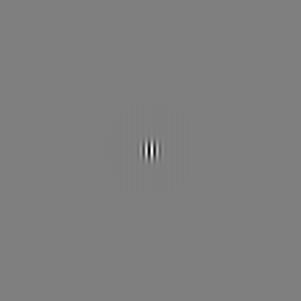
\includegraphics[width=0.11\columnwidth]{figures/rGabor0_0.jpg}
 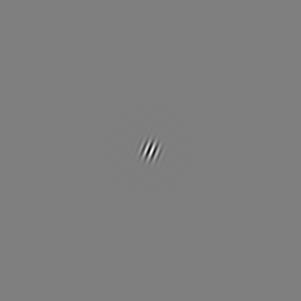
\includegraphics[width=0.11\columnwidth]{figures/rGabor0_1.jpg}
 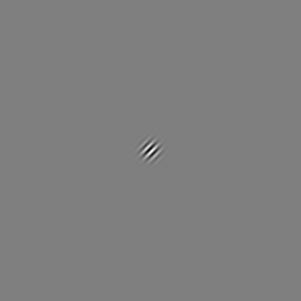
\includegraphics[width=0.11\columnwidth]{figures/rGabor0_2.jpg}
 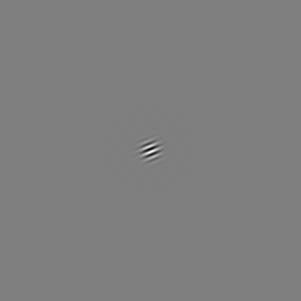
\includegraphics[width=0.11\columnwidth]{figures/rGabor0_3.jpg}
 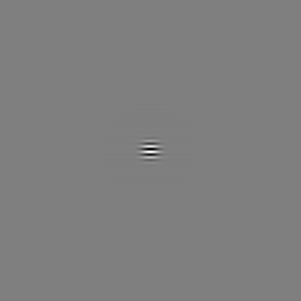
\includegraphics[width=0.11\columnwidth]{figures/rGabor0_4.jpg}
 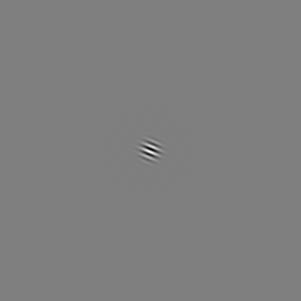
\includegraphics[width=0.11\columnwidth]{figures/rGabor0_5.jpg}
 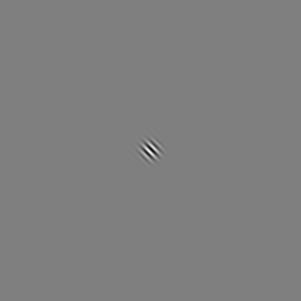
\includegraphics[width=0.11\columnwidth]{figures/rGabor0_6.jpg}
 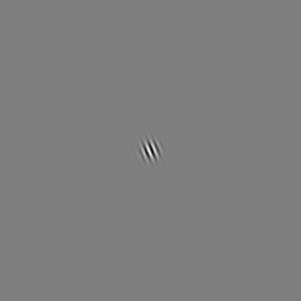
\includegraphics[width=0.11\columnwidth]{figures/rGabor0_7.jpg}\\
 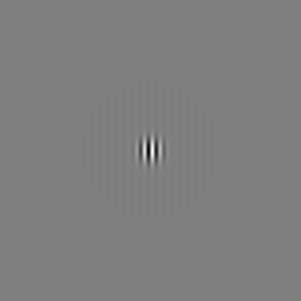
\includegraphics[width=0.11\columnwidth]{figures/rGabor1_0.jpg}
 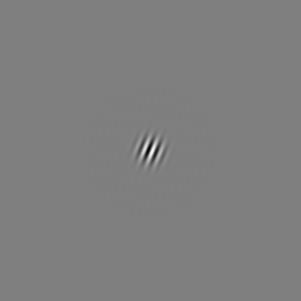
\includegraphics[width=0.11\columnwidth]{figures/rGabor1_1.jpg}
 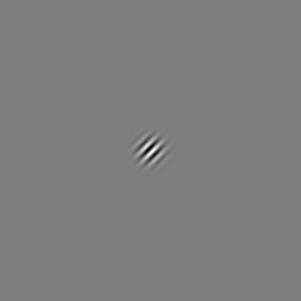
\includegraphics[width=0.11\columnwidth]{figures/rGabor1_2.jpg}
 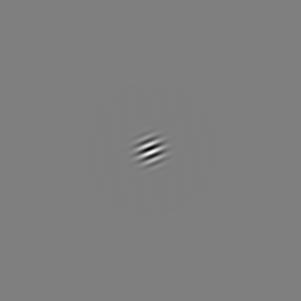
\includegraphics[width=0.11\columnwidth]{figures/rGabor1_3.jpg}
 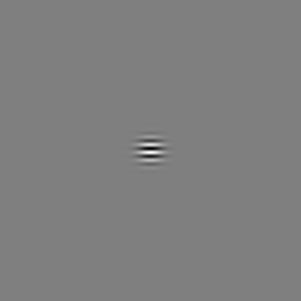
\includegraphics[width=0.11\columnwidth]{figures/rGabor1_4.jpg}
 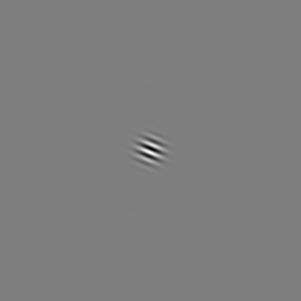
\includegraphics[width=0.11\columnwidth]{figures/rGabor1_5.jpg}
 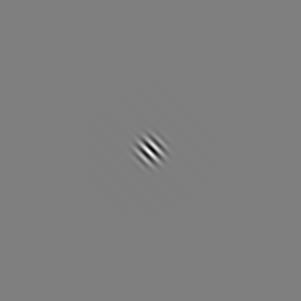
\includegraphics[width=0.11\columnwidth]{figures/rGabor1_6.jpg}
 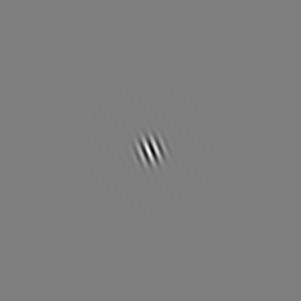
\includegraphics[width=0.11\columnwidth]{figures/rGabor1_7.jpg}\\
 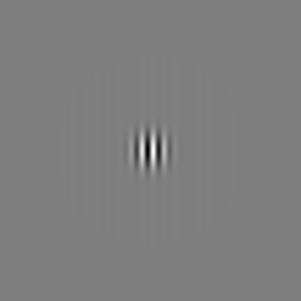
\includegraphics[width=0.11\columnwidth]{figures/rGabor2_0.jpg}
 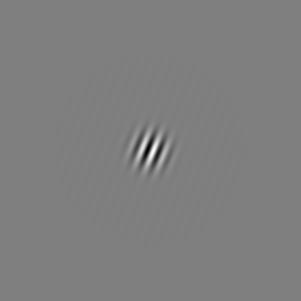
\includegraphics[width=0.11\columnwidth]{figures/rGabor2_1.jpg}
 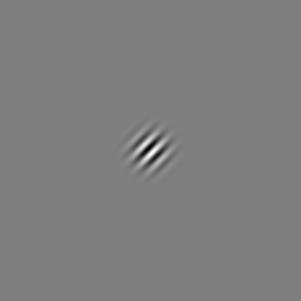
\includegraphics[width=0.11\columnwidth]{figures/rGabor2_2.jpg}
 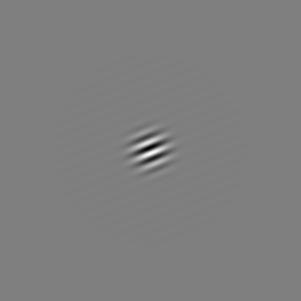
\includegraphics[width=0.11\columnwidth]{figures/rGabor2_3.jpg}
 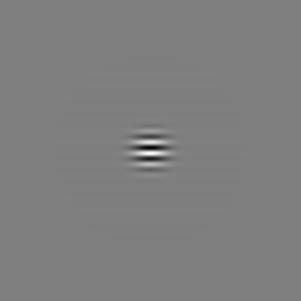
\includegraphics[width=0.11\columnwidth]{figures/rGabor2_4.jpg}
 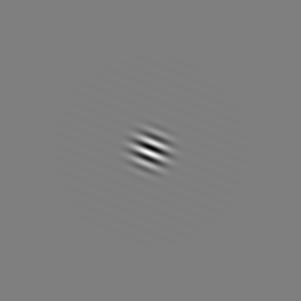
\includegraphics[width=0.11\columnwidth]{figures/rGabor2_5.jpg}
 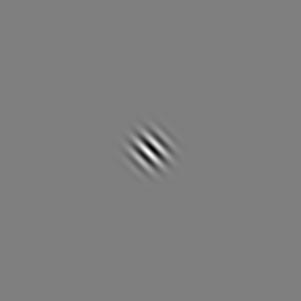
\includegraphics[width=0.11\columnwidth]{figures/rGabor2_6.jpg}
 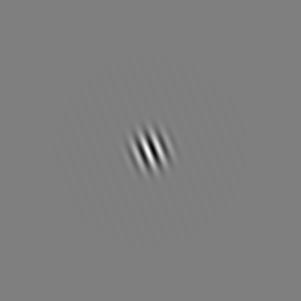
\includegraphics[width=0.11\columnwidth]{figures/rGabor2_7.jpg}\\
 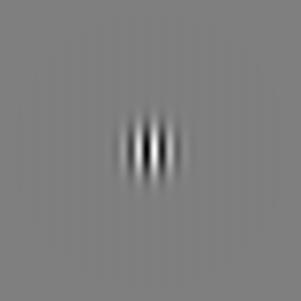
\includegraphics[width=0.11\columnwidth]{figures/rGabor3_0.jpg}
 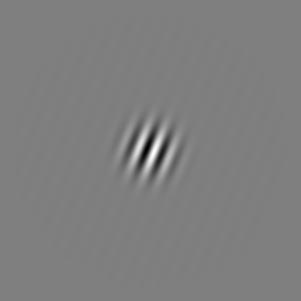
\includegraphics[width=0.11\columnwidth]{figures/rGabor3_1.jpg}
 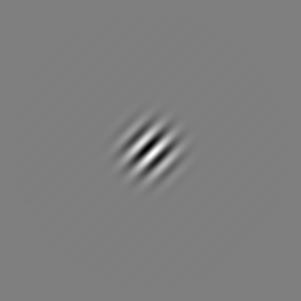
\includegraphics[width=0.11\columnwidth]{figures/rGabor3_2.jpg}
 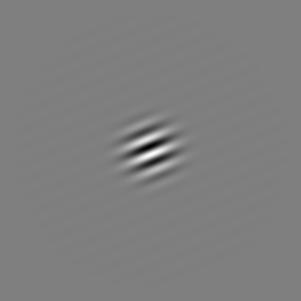
\includegraphics[width=0.11\columnwidth]{figures/rGabor3_3.jpg}
 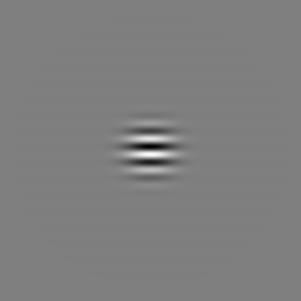
\includegraphics[width=0.11\columnwidth]{figures/rGabor3_4.jpg}
 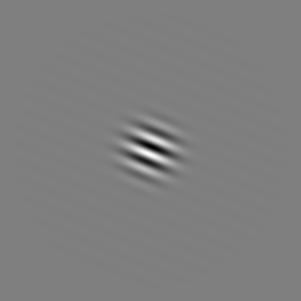
\includegraphics[width=0.11\columnwidth]{figures/rGabor3_5.jpg}
 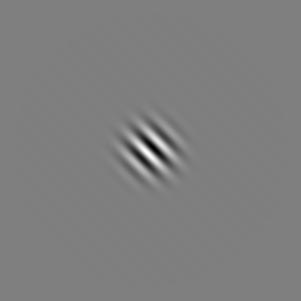
\includegraphics[width=0.11\columnwidth]{figures/rGabor3_6.jpg}
 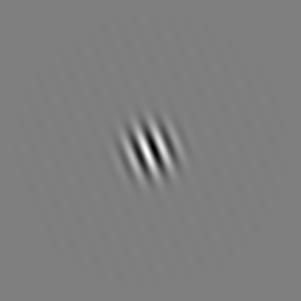
\includegraphics[width=0.11\columnwidth]{figures/rGabor3_7.jpg}\\
 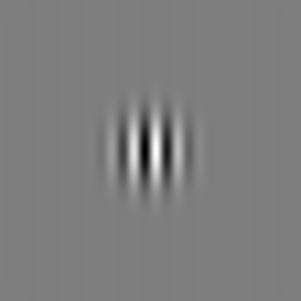
\includegraphics[width=0.11\columnwidth]{figures/rGabor4_0.jpg}
 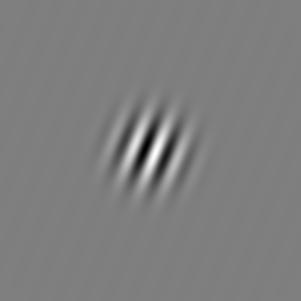
\includegraphics[width=0.11\columnwidth]{figures/rGabor4_1.jpg}
 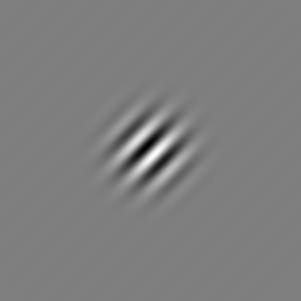
\includegraphics[width=0.11\columnwidth]{figures/rGabor4_2.jpg}
 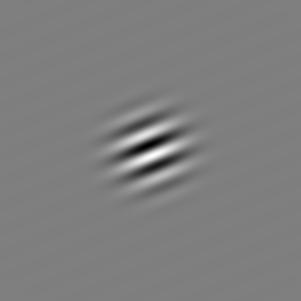
\includegraphics[width=0.11\columnwidth]{figures/rGabor4_3.jpg}
 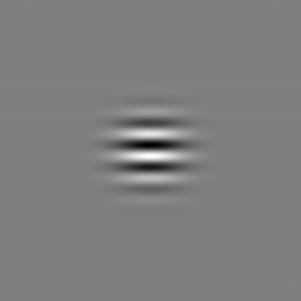
\includegraphics[width=0.11\columnwidth]{figures/rGabor4_4.jpg}
 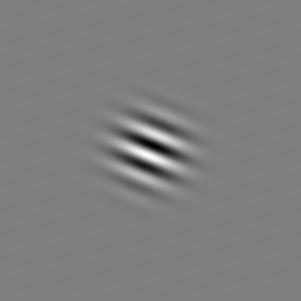
\includegraphics[width=0.11\columnwidth]{figures/rGabor4_5.jpg}
 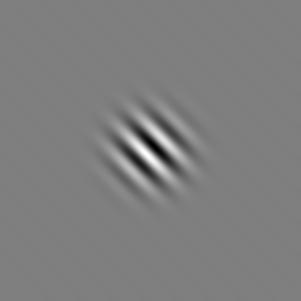
\includegraphics[width=0.11\columnwidth]{figures/rGabor4_6.jpg}
 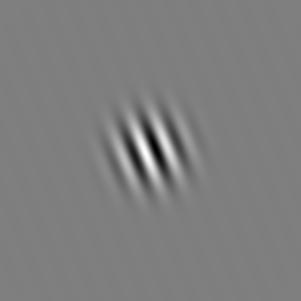
\includegraphics[width=0.11\columnwidth]{figures/rGabor4_7.jpg}\\
\caption{The real part of the $5\times8$ Gabor wavelets.}
\label{fig:realgabor}
\end{center}
\end{figure} 

\subsection{Gabor Wavelet Transform}
The Gabor wavelet representation of an image is the convolution of the image with a family of Gabor kernels as defined by \mbox{Equation} (\ref{eq:kernel}). The convolution of image $I$ and a Gabor kernel $\psi_{\mu,\nu}$ is defined as follows 
\begin{equation}\label{eq:conv}
O_{\mu,\nu}(z)=I(z)\ast\psi_{\mu,\nu}(z)
\end{equation}
The whole set of Gabor wavelet representation of the image $I(z)$ is $S=\{O_{\mu,\nu}(z):\mu\in\{0,\ldots,7\},\nu\in\{0,\ldots,4\},z=(x,y)\}$.

The response $O_{\mu,\nu}(z)$ to each Gabor kernel is a complex function with a real part $\textrm{Re}\{O_{\mu,\nu}(z)\}$ and an imaginary part $\textrm{Im}\{O_{\mu,\nu}(z)\}$ illustrated as
\begin{displaymath}
O_{\mu,\nu}(z) = \textrm{Re}\{O_{\mu,\nu}(z)\} +i\,\textrm{Im}\{O_{\mu,\nu}(z)\}
\end{displaymath}
The magnitude response $\|O_{\mu,\nu}(z)\|$ is expressed as
\begin{equation}
\|O_{\mu,\nu}(z)\| = \sqrt{\textrm{Re}\{O_{\mu,\nu}(z)\}^2 + \textrm{Im}\{O_{\mu,\nu}(z)\}^2}
\end{equation}
In this paper, the magnitude response $\|O_{\mu,\nu}(z)\|$ is used to represent the features. Therefore, a Gabor wavelet feature $j$ is configured by the three key parameters: position $z$, orientation $\mu$, and scale $\nu$, as illustrated in \mbox{Equation} \ref{eq:gaborfeature}
\begin{equation}\label{eq:gaborfeature}
j(z, \mu, \nu) = \|O_{\mu,\nu}(z)\|.
\end{equation}
For a given image $I(z)$ with $N \times M$ pixels, the number of Gabor wavelet feature representation will be $N \times M \times 40$. The feature space consists of all these features. In this case, it is 40 times larger than the original image space.



\section{Feature Selection by AdaBoost}
\label{feature_selection}
The Gabor wavelet feature representation described above resides in a very high dimensional space. It is necessary to reduce the feature space to a lower dimensional representation by feature selection. Feature selection is a technique, commonly used in machine learning and pattern recognition for reducing the dimension of a feature space. It selects a subset of relevant features from a large number of features to construct robust learning models. By removing irrelevant and redundant features from the training data, feature selection helps in improving the performance of learning models. Feature selection also helps to distinguish features which are important in learning. 

In this paper, we use AdaBoost to select significant features from the pool of Gabor wavelet features, hence to reduce the dimension. Firstly, a brief introduction to AdaBoost is given. Secondly, the key element in AdaBoost - weak learner is described and discussed. Thirdly, a novel weak learner - Potsu is proposed. Finally, there is the AdaBoost feature selection algorithm and its results conducted in the \mbox{XM2VTS} face database.

\subsection{AdaBoost}
AdaBoost (an abbreviation for Adaptive Boosting) is formulated by Freund and Schapire \cite{Freund1995} for ``boosting'' the accuracy of classification. It is a relatively efficient, simple, and easy learning strategy for improving the performance of learning algorithms by combining a set of rough and moderate learners (or classifiers). In AdaBoost, these learners are called ``weak'' learners which have low discrimination power to assign the true label correctly. Hence, AdaBoost refers to a method of combining a set of weak learners into a strong classifier which gives a high accuracy for prediction. In the term of AdaBoost, the final strong classifier is called ``ensemble'', which refers to a collection of statistical classifiers. By giving a set of examples with initial weights, AdaBoost builds an initial weak learner from the training data. It then focuses those examples in the training set which are misclassified. A new weak learner is then built with a modified training set which boosts the weights of these misclassified examples in the training process. Finally, an ensemble is combined linearly by these generated weak learners with corresponding weights to achieve higher recognition rate.

AdaBoost has been successfully applied to face detection by Viola and Jones in \cite{Viola2001}, in which images are firstly processed by \textit{integral image representation} for obtaining Haar wavelet features. Due to enormous number of Haar wavelet features, a variant of AdaBoost is used to select a small set of features and train the classifier to distinguish face or non-face. For a single feature, a weak learner is built and evaluated by the training data. In the variant of AdaBoost, an iteration is an exhaustive search on the whole set of features for the most significant features for representing faces. Each iteration selects one significant feature. The final ensemble is a combination of weak learners built on these selected features. The face detector is the most rapid and accurate face detection system compared to other systems, and it pushes face detection research and development into a new era. 

The successful AdaBoost application is used in the mode of two-class classification. Since the face verification scenario is introduced into a way of two-class classification, our face recognition algorithm also adopts AdaBoost to select significant features representing individuals. Unlike the face detection, the two classes are client and impostor. A client is the given individual with claimed identity. Impostors are all other persons except the client. In Gabor-Boosting, face images belonging to a client are defined as positive examples, and face images of impostors are defined as negative examples. In Gabor-Boosting, each client has its own feature representatives derived from AdaBoost training and classification mechanism.


\subsection{Weak learners in AdaBoost}
In AdaBoost training, the corresponding weak learner $h_{t}$ for each selected feature is collected and built into an ensemble classifier. In the original AdaBoost, the ensemble classifier is 
\begin{displaymath}
 H(x)  =  \sum_{t=1}^{T}\alpha_{t}h_{t}(x)
\end{displaymath}
where, $\alpha_{t}$ is the importance factor indicating how importantly the weak learner $h_{t}$ contributes to an ensemble classifier, and $T$ is the number of iterations (the number of weak learners in ensemble). The importance of a weak learner is evaluated by
\begin{equation}
 \alpha_{t} = \log \frac{1}{\beta_{t}}
\end{equation}
The parameter $\beta_{t}$ is defined as $\beta_{t}=\frac{\varepsilon_{t}}{1-\varepsilon_{t}}$, where the parameter $\varepsilon_{t}$ is the classification error of the selected weak learner in each iteration. The importance is also calculated by
\begin{displaymath}
 \alpha_{t} = \log \frac{1-\varepsilon_{t}}{\varepsilon_{t}}
\end{displaymath}
Because the error $\varepsilon_{t}$ of a weak learner from each iteration should be less than $1/2$, the importance $\alpha_{t}$ will be greater than zero. The smaller the error $\varepsilon_{t}$ is, the larger is the importance $\alpha_{t}$. This indicates that a weak learner with slightly ``stronger'' discriminating power, plays a more important role in the ensemble classifier to make a decision.

The training of weak learners is by finding the minimum error $\varepsilon$ with giving the training data. Such the error is evaluated by
\begin{equation}
 \varepsilon=\sum_{i=1}^{n}\omega_{t,i}|h(x_{i})-y_{i}|^{2}
\label{eq:errorwrtweights}
\end{equation}
where $\omega_{t,i}$ is the weight of example $x_i$ in the $t$-th iteration. Generally, training a weak learner is equivalent to finding a criterion which can predict labels of the training examples correctly. Different criteria could induce different results on labelling the examples, \textit{i.e.}, the number of correct predictions. Normally, a classifier is required to achieve as many correct predictions as possible. However, the aim of training a weak learner in AdaBoost is to find an optimal criterion with a different requirement, which is not the maximum prediction, but a weighted prediction.

Normally different criteria are required by different classifiers, i.e. weak learners, to meet optimal classification. Linear Discriminant Analysis (LDA) classifiers require maximising between-class variance and minimising within-class variance. Naive Bayes classifiers use the method of maximum likelihood or maximise a posterior probability. Support Vector Machine (SVM) classifiers are required to maximise the margin between classes and minimise a quantity proportional to the number of mis-classification errors. \textit{k}-nearest neighbour (\textit{k}-NN) classifiers are based on the nearest training examples in the feature space. Artificial Neural Network (ANN) classifiers are required to minimise the ratio between misclassified examples and total examples. 

The requirement for weak learner in AdaBoost training is that the training criterion must satisfy the minimal $\varepsilon$. The classifiers mentioned above, such as LDA, Naive Bayes, SVM, \textit{k}-NN, and ANN, do not satisfy the requirement. None of these classifiers can be directly introduced as the weak learner in the training, so that a new weak learner is needed.

\subsection{Potsu weak learner}
The new weak learner using an example based heuristic approach to threshold the data for AdaBoost is proposed in this section. The proposed weak learner is named \textbf{Potsu} weak learner, because it combines the concept of Perceptron with Otsu's algorithm. 

To train a weak learner rapidly, it is necessary to keep the design of weak learner as simple as possible. As a simple linear classifier, \textit{perceptron} \cite{Gallant1990} is chosen as the prototype of weak learner. A perceptron consists of observation $f_{j}$ on a feature $j$, a threshold $\theta_{j}$, and a parity $p_{j}$ as below
\begin{equation}
 h_{j}(x)=\left\{
		 \begin{array}{ll}
		  1 & \textrm{if} \quad p_{j}f_{j}(x)<p_{j}\theta_{j}\\
		  0 & \textrm{otherwise}
		 \end{array}
		\right. 
\label{eq:perceptron}
\end{equation}
The observation $f_{j}$ is numerical, hence the weak learner is dealing with one-dimensional data. The parity $p_{j}$ indicates the direction of the inequality sign, so that there are only two options for the parity $p_{j}$ - either $1$ or $-1$. The parity of Potsu weak learner is determined by comparing the mean of all positive examples with the mean of all negative examples. It is assumed when majority of positive examples are below the threshold, the parity $p_{j}$ should be equal to $1$, otherwise $-1$.

The training of a Potsu weak learner is to label examples by finding the optimal threshold $\theta_{j}$. The threshold $\theta$ should be a quantitative value within the range between the minimum and the maximum of examples' feature value $f_{j}(x)$. If there is a quantitative value $\theta'$ close to the threshold $\theta$, the error $\varepsilon'$ with respect to $\theta'$ will be also close to the minimal error $\varepsilon$ with respect to $\theta$. Since weak learners do not require ``strong'' discriminating power, it is more likely to collect a set of possible thresholds to approximate the true threshold. It is very similar to the Otsu method in which some possible thresholds are collected beforehand. These possible thresholds are called \textit{candidates}. The classification error is calculated according to each candidate, finally an optimal threshold is found with the minimum error among these candidates. A candidate $\theta'_j$ is defined between two adjacent feature values, \textit{i.e.} the mean of the two values. If there are $n$ training examples for training a Potsu weak learner, it will be $n-1$ candidates available ($\theta'_{1},\ldots,\theta'_{n-1}$). For each candidate, the accumulated error of Potsu weak learner $h$ with the candidate $\theta'_{k}$ is calculated by
\begin{equation} 
 \varepsilon'_{k} = \sum_{i=1}^{n}\omega_{i}|h(x_{i})-y_{i}|^{2}
\end{equation}
Once accumulated $\varepsilon'_{k}$ is greater than $0.5$, the calculation will stopped, because further accumulating would induce a large error which is worse than random guess \cite{Freund1995}. Finally, the candidate with the minimum error will be selected to be the threshold $\theta$. The number of candidates should be large, otherwise the candidates could not cover all possible values of threshold. On the other hand, the number should not be too large for computation.

The Potsu weak learner adopts a heuristic approach to find an optimal threshold reasonably close to the best possible solution. With a large number of examples, the accuracy on predicting the threshold is very high, due to a large number of candidates in selection. In addition, finding an optimal threshold in the Potsu weak learner is very fast due to the perceptron prototype. Perceptrons are especially suited for simple problems in pattern classification. The classification in perceptron is based on thresholding, which is one of the fastest algorithms for segmentation and recognition in pattern classification. The Potsu weak learners adopt a threshold selection technique. In this technique, the algorithm firstly is to collect a set of threshold candidates, and then evaluate the training performance on each candidate, and finally the candidate with the minimal error is selected as the optimal threshold.
The algorithm for training a Potsu weak learner is given in \mbox{Table} \ref{tab:potsu}. In \cite{Friedman2000,LiStan2004,Schapire1998}, weak learners are modeled as the log likelihood ratio (LLR), which requires to predict probability density functions. Obviously, a Potsu weak learner is faster than those LLR based weak learners which demand the complicated prediction on the probability density function.
\begin{table}[h]
\caption{The algorithm for training Potsu weak learners}
\begin{tabular}{p{\columnwidth}}
\hline
\begin{algorithmic}[1]
\STATE Given a feature $j$ and example $(x_{1},y_{1}),\ldots,(x_{n},y_{n})$ and $y_{i} \in Y=\{0,1\}$ for negative and positive respectively, $f_{j}(x)$ is the value of the feature $j$ on the example data $x$. For an example $(x_{i},y_{i})$, a weight $\omega_i$ is given.
\STATE Construct a Potsu weak learner according to \mbox{Equation} \ref{eq:perceptron}.
\STATE Calculate the mean feature value $\bar{\mu}_{1}$ on all positive examples and the mean feature value $\bar{\mu}_{0}$ on all negative examples 
\IF{$\bar{\mu}_{1}<\bar{\mu}_{0}$}
	\STATE the parity $p=1$
\ELSE
	\STATE the parity $p=-1$
\ENDIF
\STATE Sort all $f_{j}(x_{i})\quad i \in \{1,\ldots,n\}$ into $f'_{j}(x_{1}),\ldots,f'_{j}(x_{n})$
\FOR{every two adjacent sorted examples $f'_{j}(x_{i})$ and $f'_{j}(x_{i+1})$}
	\STATE Compute the $i$th candidate $\theta'_{i}=\frac{f'_{j}(x_{i})+f'_{j}(x_{i+1})}{2}$.
\ENDFOR
\FORALL{$n-1$ candidates $\theta'_{1},\ldots,\theta'_{n-1}$}
	\STATE Suppose $\theta'_{k}$ as the threshold $\theta_{j}$ in \mbox{Equation} \ref{eq:perceptron}.
	\STATE Calculate the error $\varepsilon'_{k} = \sum_{i=1}^{n}\omega_{i}|h_{j}(x_{i})-y_{i}|^{2}$ with respect to  $\omega_{i}$.
	\IF{$\varepsilon'_{k} >0.5$}
		\STATE reject the candidate $\theta'_{k}$.
	\ENDIF
\ENDFOR
\STATE Select the corresponding candidate $\theta'_{j}$ with the lowest error $\varepsilon$ as the threshold $\theta_{j}$.
\STATE A trained Potsu weak learner is $h_{j}(x)=\left\{
		 \begin{array}{ll}
		  1 & \textrm{if} \quad pf_{j}(x)<p_{j}\theta_{j}\\
		  0 & \textrm{otherwise}
		 \end{array}
		\right.$
\end{algorithmic}\\
\hline
\end{tabular}
\label{tab:potsu}
\end{table}




\subsection{Boosting Feature Selection}
The algorithm of AdaBoost is presented in \mbox{Table} \ref{tab:binarygaborboosting} for Gabor wavelet feature selection. AdaBoost maintains weights $\omega_{t}$ as a probability distributed over training examples. The weights represent how hard the corresponding examples to be recognised correctly. At the beginning, the weights belonging to a same class (either client or impostor) are set equally. In the course of iteration, the weights are updated according to the performance of the selected weak learner. If an example is recognised incorrectly by the weak learner, the corresponding weight increases (indicating the example is hard to be recognised), and vice versa.
\begin{table}[ht]
\caption{Feature selection algorithm}
\begin{tabular}{p{\columnwidth}}
\hline
\begin{algorithmic}[1]
{
\STATE Given example $(x_{1},y_{1}),\ldots,(x_{n},y_{n})$, where $x_{i}$ is the data of the $i$th example, which consist of $k$ features $\{j_{1},\ldots,j_{k}\}$, and $y_{i} \in Y=\{0,1\}$ for negative examples and positive examples respectively..
\STATE Initialise the weights $\omega_{1,i}=\frac{1}{2m},\frac{1}{2l}$ for $y_{i}=0,1$ respectively, where $m$ and $l$ are the number of negative and positive examples respectively.
\FOR{$t=1,\ldots,T$}
	\STATE Normalise the weights, $\omega_{t,i}\leftarrow\frac{\omega_{t,i}}{\sum_{i=1}^{n}\omega_{t,i}}$ so that $\omega_{t,i},i=\{1,\ldots,n\}$ form a probability distribution.
	\FORALL{$\{j_{1},\ldots,j_{k}\}$}
		\STATE Train a  weak learner $h_{j}$ built with one single feature $j$ with the weights $\omega_{t,i}$.
		\STATE The error is calculated as $\varepsilon_{j}=\sum_{i=1}^{n}\omega_{t,i}|h_{j}(x_{i})-y_{i}|^{2}$ with respect to $\omega_{t,i}$
	\ENDFOR
	\STATE Choose the optimal weak learner $h_{t}$ with the lowest error $\varepsilon_{t}$ from all $h_{j}$.
	\STATE Select the corresponding feature $j_{t}$ of the weak learner $h_{t}$ as a significant feature.
	\STATE Remove the feature $j_{t}$ from the feature set $\{j_{1},\ldots,j_{k}\}$.
	\STATE Update the weights $\omega_{t+1,i}=\omega_{t,i}\beta_{t}^{1-e_{i}}$, where $e_{i}=0$ if example $x_{i}$ is classified correctly and $e_{i}=1$ otherwise, and $\beta_{t}=\frac{\varepsilon_{t}}{1-\varepsilon_{t}}$.
	\STATE Choose the importance $\alpha_{t}=\log\frac{1}{\beta_{t}}$, and $\beta_{t}=\frac{\varepsilon_{t}}{1-\varepsilon_{t}}$.
\ENDFOR
\STATE The ensemble classifier
\begin{displaymath}
 H(x)  = 
		\left\{
		 \begin{array}{ll}
		  1 & \sum_{t=1}^{T}\alpha_{t}h_{t}(x) \geq \frac{1}{2}\sum_{t=1}^{T}\alpha_{t}\\
			\\
		  0 & \textrm{otherwise}
		 \end{array}
		\right. 
\end{displaymath}
}
\end{algorithmic}\\
\hline
\end{tabular}
\label{tab:binarygaborboosting}
\end{table}

In the AdaBoost training, a weak learner is constructed upon a single feature, so that there are numerous weak learners representing all features. In each iteration, all weak learners are evaluated by the training set. A weak learner with the minimum error $\varepsilon_{t}$ is selected, and its corresponding feature is selected as a significant feature. If the training has $T$ iterations, $T$ features are selected from the original feature set.

The basic idea of Boosting is to use a group of weak learners to construct a strong classifier, such that the ensemble classifier $H(x)$ is a linear combination of selected weak learners $h_t(x)$ with the corresponding importance $\alpha_t$. The factor $\alpha_t$ specifies how important the corresponding weak learner is in making decision of $H(x)$.

The experiment is carried out on eight clients from the \mbox{XM2VTS} face database. A small group of features are selected for each client. For each client, the first four images are taken for training, and the other four images are for testing. For $200$ clients, the training set has $800$ face images, and the testing set has $1560$ face images\footnote{$200$ clients with $4$ images and $95$ impostors with $8$ images}. Given a specific client in the training set, four images belong to the client, and the other $796$ images are impostors. The ratio between the number of positive and negative examples is $4:796$. Inside the \mbox{XM2VTS}, an image size is of $25\times24$ pixels. Each image is convolved with $40$ Gabor wavelets. Consequently, the total number of features for each image is $25\times24\times40=24,000$.  In each iteration, a large number of features are rejected by control the error $\varepsilon$. If the error $\varepsilon$ exceeds $0.5$, the corresponding feature will be rejected and not taken into the next iteration.

After AdaBoost feature selection, a small set of features are selected as significant features for the eight clients in \mbox{XM2VTS}. The number of selected features from each client is different. From the 1st client to the 8th client, the number of selected features are varying from 30 to 80. \mbox{Figure} \ref{fig:resultBGC1toC8full} displays these selected features projected on the corresponding client face image in the top row and the first Gabor wavelet features for each client in the bottom row. 
\begin{figure}[ht]
 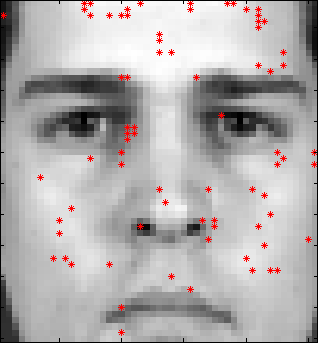
\includegraphics[width=\textwidth*11/100]{figures/XM2VTS_Full_1.png}
 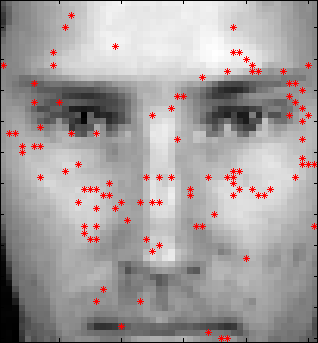
\includegraphics[width=\textwidth*11/100]{figures/XM2VTS_Full_2.png}
 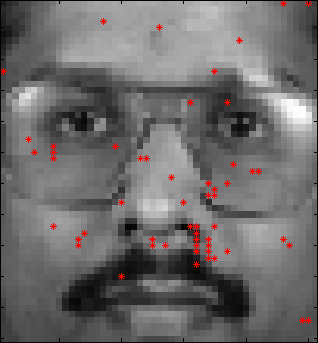
\includegraphics[width=\textwidth*11/100]{figures/XM2VTS_Full_3.png}
 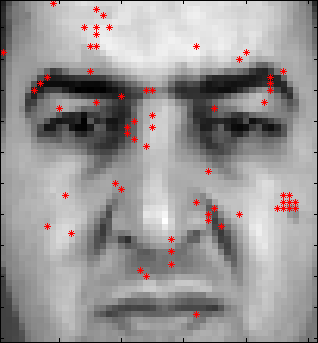
\includegraphics[width=\textwidth*11/100]{figures/XM2VTS_Full_4.png}
 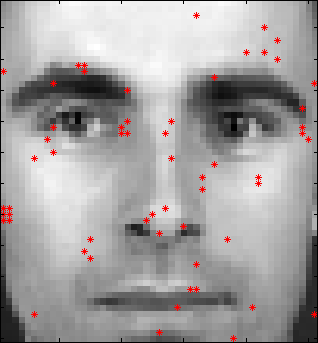
\includegraphics[width=\textwidth*11/100]{figures/XM2VTS_Full_5.png}
 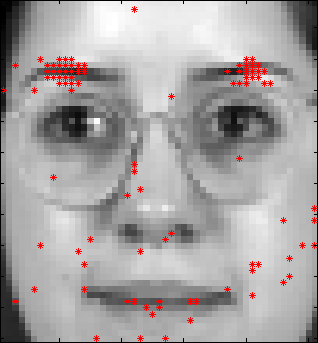
\includegraphics[width=\textwidth*11/100]{figures/XM2VTS_Full_6.png}
 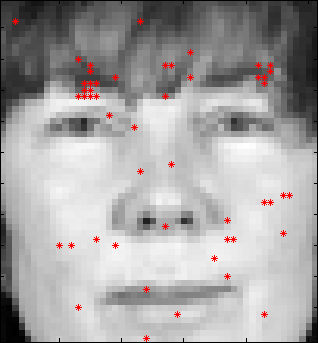
\includegraphics[width=\textwidth*11/100]{figures/XM2VTS_Full_7.png}
 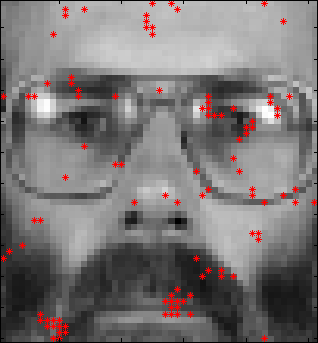
\includegraphics[width=\textwidth*11/100]{figures/XM2VTS_Full_8.png}\\
 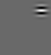
\includegraphics[width=\textwidth*11/100]{figures/firstgabor_Full_1.png}
 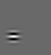
\includegraphics[width=\textwidth*11/100]{figures/firstgabor_Full_2.png}
 \includegraphics[width=\textwidth*11/100]{figures/firstgabor_Full_3.png}
 \includegraphics[width=\textwidth*11/100]{figures/firstgabor_Full_4.png}
 \includegraphics[width=\textwidth*11/100]{figures/firstgabor_Full_5.png}
 \includegraphics[width=\textwidth*11/100]{figures/firstgabor_Full_6.png}
 \includegraphics[width=\textwidth*11/100]{figures/firstgabor_Full_7.png}
 \includegraphics[width=\textwidth*11/100]{figures/firstgabor_Full_8.png}
\caption{The selected features on face images and the first selected Gabor wavelet feature.}
\label{fig:resultBGC1toC8full}
\end{figure} 
It has been noticed that these selected features are randomly distributed on faces, and they are also distributed on common facial feature areas, such as eyes, eyebrows, nose, and mouth. Interestingly, there are features located on the mole of the 4th client's face. 






\section{Classification}
\label{classification}
After feature selection, an ensemble classifier is spontaneously reminded as the classification solution. In the first part of this section, the recognition results from the ensemble solution is presented, and exhibits with overfitting. Hence, in the second part of this section, an alternative classifier - SVM is used to reduce overfitting. It shows that SVM is appropriate for Gabor-Boosting face recognition algorithm.

\subsection{Ensemble classification}
In the \mbox{XM2VTS} face database, the features are selected and the ensemble classifiers are built for each client. The classification results of the ensemble classifier $H$ from the first client to the eighth client are shown in \mbox{Table} \ref{tab:normalresultsclassify}.
\begin{table}
\caption{The classification performance of AdaBoost Classifier}
\begin{center}
 \begin{tabular}{|c|c|c|c|c|c|}
  \hline
  Client & Number & \multicolumn{2}{c|}{Training Set (\%)} & \multicolumn{2}{c|}{Testing Set (\%)}\\
  \cline{3-6}
  No & of Features & $ \mathcal{FN}$ & $ \mathcal{FP}$ & $ \mathcal{FN}$ & $ \mathcal{FP}$ \\
  \hline
  1 & 48 & 0.0 & 0.0 & 100 & 0.0 \\
  2 & 74 & 0.0 & 0.0 & 100 & 0.0 \\
  3 & 37 & 0.0 & 0.0 & 100 & 0.0 \\
  4 & 44 & 0.0 & 0.0 & 100 & 0.0 \\
  5 & 48 & 0.0 & 0.0 & 75 & 0.0 \\
  6 & 57 & 0.0 & 0.0 & 100 & 0.0 \\
  7 & 40 & 0.0 & 0.0 & 100 & 0.0 \\
  8 & 75 & 0.0 & 0.0 & 100 & 0.0 \\
  \hline
 \end{tabular} 
\label{tab:normalresultsclassify}
\end{center}
\end{table} 
All ensemble classifiers have the best performance on the training set, where all classifiers have achieved zero error, \textit{i.e.}, no mis-classification. Both false positive rate $\mathcal{FP}$ and the false negative rate $\mathcal{FN}$ are equal to zero so that the ensemble classifiers have achieved the perfect results in the training set. However, in the testing set, the ensemble classifiers reveal poor classification performance on positive examples, i.e. high $\mathcal{FN}$. Most positive examples are misclassified except the 5th client, but all negative examples are classified correctly.

Experimental results suggest the performance of the ensemble classifier on the training set does not represent its overall performance. The ensemble classifier is trained to perform perfectly on the training set, but reveals poor performance on other data sets, \textit{e.g.}, the testing set. This phenomenon is so called \textit{overfitting}. The overfitting is a wide research topic in pattern recognition, machine learning, data mining, etc. There are many issues that lead to overfitting. In this case, the issues causing the overfitting are categorised into two main sources: inferior training data and classification algorithm.

The inferior training data may lead to overfitting. Inside this source, the reason is \textbf{curse of dimensionality}. The overfitting in this case is partly due to the small number of positive examples in the training set. Generally, the number of training examples is related to the number of features used in classification. In \cite{Jain2000}, it is stated that the number of training examples per class should be at least ten times the number of features. If the number of training examples does not satisfy this requirement, the performance of classification will be degraded. This phenomenon is called ``curse of dimensionality''. The number of features used in the classification is around $30$ to $80$. The number of training examples per class should be around $300$ to $800$. In this case, the number of training examples of positive class is only four, which is far less than the required number. 

A phenomenon that AdaBoost is prone to overfit has been observed in \cite{Grove1998,Mason1999}. In \cite{Opitz1999}, it concludes that ensemble classifiers in AdaBoost may suffer from overfitting in the presence of noise which may explain some of the decreases in performance. Inside the source, there are two issues pertinent to overfitting. The first issue is that the AdaBoost training over-emphasises noisy examples, and the second issue is due to the weighted voting used by ensemble classifiers. Freund and Schapire \cite{Freund1996} suggested that the poor performance of AdaBoost ensemble classifier results from overfitting the training dataset since later training may be over emphasising examples which are actually noise. In AdaBoost, an example with a higher weight is more emphasised in the training than other examples with lower weights. After each iteration of AdaBoost, the weights of some mis-classified examples are increased. In the next iteration, the training will place more emphasise on these examples which are often referred to as ``hard'' examples. However, if these ``hard'' examples include high level noise, the AdaBoost training learns the noise rather than the nature of the data itself. For a problem with noise, focusing on misclassified examples may cause the ensemble classifier to focus on boosting the margins of noise, but not on boosting the margins of examples. In fact, the weight updating misleads the AdaBoost training in overall classification. In \cite{Opitz1999}, noises from different levels are added into data sets, and the results demonstrate the error rate of the AdaBoost may indeed increase as the number of weak learners increases. In \cite{Schapire1997}, it suggests that later weak learners focus on increasing the margins for examples. Early stop is useful in AdaBoost training for the purpose of increasing performance. Within the ensemble classifier, each weak learner is associated with an importance $\alpha_t$, which is also considered as a weight for that weak learner. Hence, the output of ensemble classifier is the combination of weighted voting from all weak learners. Previous work \cite{Sollich1995} has shown how different weight voting schemes can generally be resilient or lead to overfitting. In the work, optimising the weights is the method of choice for achieving minimal generalisation error. In general, uniformly distributed weights may cause the overfitting, while with optimised weights the ensemble classification is insensitive to overfitting.


\subsection{SVM classification}
Since AdaBoost is prone to the overfitting, an alternative classifier - SVM is used to classify the examples. In this section, an SVM classifier is trained with the given selected features on the training set.

SVMs are a collection of learning approaches used for generalised linear or non-linear classification. SVMs are to minimise the classification error and maximise the geometric margin, so that SVMs are also known as maximum margin classifiers. For two-class classification, it is assumed that there is a hyperplane (also called a \textit{decision boundary}) separating the clusters of two classified data. SVMs project input vectors to a higher dimensional space where a maximal separating hyperplane is created. The separating hyperplane maximises the distance between the two classes. An assumption is made that the larger the margin or distance between two classes, the lower the generalisation error of the classifier will be. The original optimal hyperplane algorithm is a linear classifier. However,  non-linear SVMs can be created by applying the kernel method \cite{Taylor2004} to maximum-margin hyperplanes. The algorithm is allowed to fit the maximum-margin hyperplane in the modified feature space. The classifier is a hyperplane in the high-dimensional feature space, which may be non-linear in the original input space. The kernels can be adopted as a polynomial kernel, a radial based kernel, or a Gaussian radial basis kernel. In this paper, a Matlab SVM toolbox - OSU Support Vector Machines (SVMs) Toolbox \cite{Ma2001} is used to perform the task of classification.

Experiments are also carried out on the eight clients from the XM2VTS. A non-linear SVM classifier with a polynomial kernel of degree three is constructed from the $800$ training examples, which are the first four images across 200 clients.

Freund and Schapire \cite{Freund1996} suggest that AdaBoost training emphasises on noisy examples at the later iterations, so that the overfitted result is acquired at the end of training. The training of SVM is the optimisation process which is to find the primal form of the Lagrange formalism. By optimising the Lagrange function, a small group of Support Vectors (SVs) are obtained, which defines the hyperplanes between classes. The SVs are examples with non-zero Lagrange multipliers. In this case, $5$ to $11$ examples are taken as SVs from totally $800$ training examples. The number of SVs for the eight clients is shown in \mbox{Table} \ref{tab:noSVs}. 
\begin{table}[ht]
\begin{center}
\caption{Number of SVs in the SVMs based on the eight clients}
 \begin{tabular}{|c|c|c|c|}
  \hline
  Client & No of SVs & No of Positive SVs & No of Negative SVs \\
  \hline
  1 & 7 & 1 & 6 \\
  2 & 11 & 2 & 9 \\
  3 & 5 & 1 & 4 \\
  4 & 10 & 1 & 9 \\
  5 & 9 & 1 & 8 \\
  6 & 7 & 1 & 6 \\
  7 & 7 & 2 & 5 \\
  8 & 5 & 2 & 3 \\
  \hline
 \end{tabular}
\label{tab:noSVs} 
\end{center}
\end{table}
Hence, SVMs use a small number of examples to construct classifiers instead of the whole set of examples (including the noisy examples). This optimisation process is equivalent to finding some examples, \textit{i.e.}, SVs, which contain the lowest level of noise. By only using SVs, noisy examples are excluded in the construction of classifier. The training and classification only emphasise on those examples with the lowest level of noise, so that the overfitting caused by noisy data is reduced to the minimum level. In addition, when SVMs are designed originally, the overfitting issues are taken into account. SVMs avoid overfitting by choosing a specific hyperplane among the many that can separate the data in the feature space. SVMs find the maximum margin hyperplane, which maximises the minimum distance from the hyperplane to the closest SVs.

The training process of SVM is to find a linear discriminant function
\begin{equation}
 g(x)=\mathbf{\omega}^T \mathbf{x} + b
\end{equation}
where $\mathbf{x}$ is the vector $\{x_1,x_2,\ldots,x_n\}$ from $n$ features, $\mathbf{\omega}$ is the weight vector $\{\omega_1,\omega_2,\ldots,\omega_n\}$ for corresponding $n$ features, and $b$ is a bias. The weights also imply how importantly the corresponding features play roles in classification. When these weights are normalised into a probability distribution, the weights vary dramatically. The probability distributions of weights from eight clients are shown in \mbox{Figure} \ref{fig:weightdistc1toc8}. For SVMs, a few features have their weights much higher than others. This indicates that only a small number of features play more important roles in classification. However, in ensemble classification the weights (\textit{i.e.} importance $\alpha_{t}$) for each feature are distributed nearly uniformly. Hence, when the weights for selected features are optimised, the overfitting effect is reduced in SVMs.
\begin{figure}
\begin{center}
  \subfigure[The 1st client]{\includegraphics[width=170pt,height=88pt]{figures/C1_SVM.jpg}}
  \subfigure[The 2nd client]{\includegraphics[width=170pt,height=88pt]{figures/C2_SVM.jpg}}
  \subfigure[The 3rd client]{\includegraphics[width=170pt,height=88pt]{figures/C3_SVM.jpg}}
  \subfigure[The 4th client]{\includegraphics[width=170pt,height=88pt]{figures/C4_SVM.jpg}}
  \subfigure[The 5th client]{\includegraphics[width=170pt,height=88pt]{figures/C5_SVM.jpg}}
  \subfigure[The 6th client]{\includegraphics[width=170pt,height=88pt]{figures/C6_SVM.jpg}}
  \subfigure[The 7th client]{\includegraphics[width=170pt,height=88pt]{figures/C7_SVM.jpg}}
  \subfigure[The 8th client]{\includegraphics[width=170pt,height=88pt]{figures/C8_SVM.jpg}}
\end{center}
 \caption{The weight distribution on eight clients of XM2VTS}
\label{fig:weightdistc1toc8}
\end{figure} 

After the SVM classifiers are trained, the training set and the testing set are given for the testing purpose. \mbox{Table} \ref{tab:svmevaluation} shows the performance of SVM classification belonging to eight clients.
\begin{table}[ht]
\caption{The performance of SVM classification on eight clients with all selected features}
 \begin{center}
   \begin{tabular}{|c|c|c|c|c|c|}
  \hline
    & Number of &\multicolumn{2}{c|}{Training Set (\%)} & \multicolumn{2}{c|}{Testing Set (\%)}\\
   \cline{3-6}
  Client & Features &$\mathcal{FN}$ & $\mathcal{FP}$ & $\mathcal{FN}$ & $\mathcal{FP}$ \\
  \hline
  1 & 48 & 0.0 & 0.0 & 0.0 & 0.0\\
  2 & 74 & 0.0 & 0.0 & 0.0 & 0.06\\
  3 & 37 & 0.0 & 0.0 & 50 & 0.0\\
  4 & 44 & 0.0 & 0.0 & 0.0 & 0.0\\
  5 & 48 & 0.0 & 0.0 & 0.0 & 0.0\\
  6 & 57 & 0.0 & 0.0 & 0.0 & 0.0\\
  7 & 40 & 0.0 & 0.0 & 100 & 0.13\\
  8 & 75 & 0.0 & 0.0 & 100 & 0.0\\
  \hline
 \end{tabular}
 \end{center}
\label{tab:svmevaluation}
\end{table} 
On the 1st, 2nd, 4th, 5th and 6th clients, SVMs achieve perfect performance, i.e. zero error. All positive examples in both the training set and the testing set are classified correctly. For the 2nd client, only one negative example is falsely recognised as positive, and the false positive rate $\mathcal{FP}$ is $0.06\%$ which is very small and can be neglected. Hence, the SVM can achieve low error rate comparing with \mbox{Table} \ref{tab:normalresultsclassify}, the result from SVM reveals the better performance than ensemble classifier.

\subsection{Summary}
Both inferior training dataset and ensemble classifier in AdaBoost lead to overfitting. When the classifier is changed to SVM, the performance of classification improves for some clients, which demonstrates using an SVM classifier is an appropriate choice for classification. In the real implementation under a restricted face database, it is impossible to improve the training dataset, i.e. impossible to increase the number of examples per class. Hence, the only way to solve overfitting is to use alternative classifiers, such as SVM. In the proposed algorithm, significant features are selected by AdaBoost algorithm, while the verification is performed by SVM.

\section{Conclusion}
\label{conclusion}
In this paper, a highly accurate appearance-based grey scale frontal face recognition algorithm - Gabor-Boosting face recognition, is presented. The strong recognition performance in the face recognition is highlighted by \textit{Gabor wavelet transform}, \textit{AdaBoost}, \textit{Support Vector Machine (SVM)}. The Gabor wavelets are of similar shape as the receptive fields of simple cells in the primary visual cortex, and demonstrate significant potential in biometrics such as iris recognition and face recognition. AdaBoost is one of the most successful and popular learning algorithms. The classification is designed to construct a ``strong" classifier from ``weak'' learning algorithms. The SVM is a powerful learning algorithm for solving a variety of learning and function estimation problems, such as pattern recognition and regression estimation. The SVM provides non-linear classification by mapping the input into high-dimensional feature space where a special type of hyperplane is constructed. The overall recognition performance is benefited by the combination of the three key components. The Gabor wavelet transform extracts features which describe texture variations in human faces. The AdaBoost algorithm selects the most significant features which represent different individuals. The SVM constructs a hyperplane for classification with respect to selected features. In the AdaBoost feature selection, a heuristic example-based weak learner - Potsu weak learner is proposed. Potsu weak learner takes the perceptron as its prototype, and use a heuristic thresholding technique to learn decision rules from examples in training data. 

The Gabor-Boosting face recognition algorithm is robust under small number of example images per subject in training data. In the situation of small number of positive examples, the system has achieved nearly $0$ false positive rate and moderate false negative rate. Potential applications of the algorithm are possibly in highly secure face authentication systems dedicated to a small group of clients. The systems thus have ``no false detections on impostors'' and ``an appropriate acceptance detection rate on clients''.
 
\bibliographystyle{plain}
\bibliography{GaborBoosting}
\end{document}
